\documentclass{beamer}
\usetheme{metropolis}           % Use metropolis theme

\usepackage{tikz}
\usepackage[utf8]{inputenc}
\usepackage[spanish]{babel}

\usepackage{smartdiagram}
\usepackage{qtree}
\usepackage{verbatim}
\usepackage{svg}
\usepackage{graphicx}
\usepackage{color}
\definecolor{lightgray}{rgb}{0.95, 0.95, 0.95}
\definecolor{darkgray}{rgb}{0.4, 0.4, 0.4}
%\definecolor{purple}{rgb}{0.65, 0.12, 0.82}
\definecolor{editorGray}{rgb}{0.95, 0.95, 0.95}
\definecolor{editorOcher}{rgb}{1, 0.5, 0} % #FF7F00 -> rgb(239, 169, 0)
\definecolor{editorGreen}{rgb}{0, 0.5, 0} % #007C00 -> rgb(0, 124, 0)
\definecolor{orange}{rgb}{1,0.45,0.13}		
\definecolor{olive}{rgb}{0.17,0.59,0.20}
\definecolor{brown}{rgb}{0.69,0.31,0.31}
\definecolor{purple}{rgb}{0.38,0.18,0.81}
\definecolor{lightblue}{rgb}{0.1,0.57,0.7}
\definecolor{lightred}{rgb}{1,0.4,0.5}
\usepackage{upquote}
\usepackage{listings}
\lstset{language=html,
	basicstyle=\footnotesize\ttfamily,
	keywordstyle=\footnotesize\color{blue}\ttfamily,
}

\usebackgroundtemplate%
{%
	
\includegraphics[width=\paperwidth]{Images/fondo}%
}

\title{Microservicios funcionales con Java 8 y Java EE}
\author{Víctor Orozco - @tuxtor}
\institute{Java Cloud Day Mexico 2017}
\date{\today}

\begin{document}

\frame{\titlepage}

\begin{frame}{Acerca de}
\begin{figure}
	\centering
	
\includegraphics[width=\linewidth]{Images/fescudos}
\end{figure}
\end{frame}

\begin{frame}{Advertencia 1}
\huge Esta presentación se basa exclusivamente en mi búsqueda diaria por trabajar menos, proyectos fracasados, lecciones aprendidas, poco capital y mucho código ;-)
\end{frame}

\begin{frame}{Advertencia 1}
¿Estado zen del arquitecto de software?
\begin{figure}
	\centering
	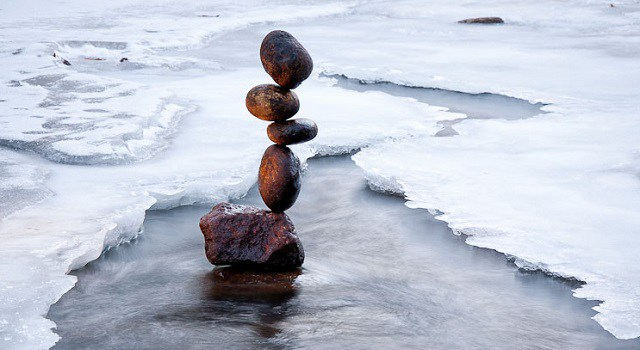
\includegraphics[width=\linewidth]{Images/zen}
\end{figure}
\end{frame}

\begin{frame}{Advertencia 1}
Estado zen del arquitecto de software
\begin{itemize}
	\item Productividad
	\item Recurso humano
	\item Predictibilidad y estabilidad
	\item Escalabilidad
	\item Costos
\end{itemize}
\end{frame}

\begin{frame}{Advertencia 1}
Estado zen del arquitecto de software
\begin{itemize}
	\item Productividad - Java 8
	\item Recurso humano - POO -> Funcional
	\item Predictibilidad y estabilidad - Java EE 7
	\item Escalabilidad brutal - Microservicios
	\item Costos - Todas las anteriores
\end{itemize}
\end{frame}

\begin{frame}{Advertencia 1}
Estado zen del arquitecto de software
\begin{itemize}
	\item \textbf{Productividad} - Java 8
	\item Recurso humano - POO -> Funcional
	\item \textbf{Predictibilidad y estabilidad} - Java EE 7
	\item \textbf{Escalabilidad brutal} - Microservicios
	\item Costos - Todas las anteriores
\end{itemize}
\end{frame}

\begin{frame}{Microservicio funcional}
\huge TL;DR Microservicio creado con programación funcional
\end{frame}

\begin{frame}{Microservicio funcional . . . con Payara Micro}
\huge TL;DR Microservicio creado con Java 8, algunas APIs de JavaEE y Payara Micro
\end{frame}

\section{Java 8}
\begin{frame}{Java 8}
     \begin{columns}[T] % contents are top vertically aligned
	     \begin{column}[T]{5cm} % each column can also be its own environment
				\begin{itemize}
				\item Nashorn
				\item Date/Time API
				\item Compact Profiles
				\item Type Annotations
				\item \textbf{Default methods}
				\item \textbf{Streams}
				\item \textbf{Lambda Expressions}
				\end{itemize}
	     \end{column}
	     \begin{column}[T]{5cm} % alternative top-align that's better for graphics
			\begin{figure}
			\centering
			
\includegraphics[width=0.7\linewidth]{Images/JavaLam-1}
			\end{figure}

	     \end{column}
     \end{columns}
\end{frame}


\begin{frame}{Paradigmas (Simplificación)}

\Tree[.Paradigmas [.Imperativo [.Estructurado \textit{Pascal} ]
               [.\alert{OOP}  \textit{Java} ]]
          [.Declarativo [.\alert{Funcional} \textit{Clojure} ]
                [.Logico \textit{Prolog} ]]]
\end{frame}

\begin{frame}{Programación funcional}
	\begin{itemize}
	\item Computación = Evaluación de funciones matemáticas (calculo de lambdas)
	\item NO cambios en estado
	\item NO mutar datos
	\item Declarativo $\to$ Expresiones 
	\end{itemize}
\end{frame}

\begin{frame}{Java 8}
Un lenguaje de programación orientada a objetos con características funcionales.
			\begin{figure}
			\centering
			
\includegraphics[width=0.5\linewidth]{Images/JavaLam-1}
			\end{figure}
\end{frame}

\begin{frame}{¿Porque programación funcional?}
	\begin{itemize}
	\item Paralelismo
	\item Multicore, multicpu
	\item \textbf{Elegancia}
	\end{itemize}
\end{frame}

\begin{frame}{Programación funcional en Java 8}
	\begin{itemize}
	\item Java no es un lenguaje funcional puro (Clojure)
	\item Otras opciones JVM (Scala, Kotlin, Ceylon)
	\item Java soporta programación funcional a través de \textbf{bibliotecas}
	\end{itemize}
\end{frame}

\section{Código funcional}
\begin{frame}{PF en Java (Consecuencias)}
\begin{figure}
	\centering
	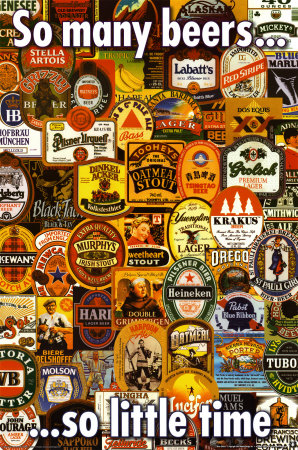
\includegraphics[width=0.45\linewidth]{Images/somany}
\end{figure}
\end{frame}

\begin{frame}{PF en Java (Consecuencias)}
\huge Java 8 generó un nuevo ecosistema de bibliotecas funcionales, declarativas y reactivas . . .
\end{frame}

\begin{frame}{PF en Java (Consecuencias)}
Google: Como me vuelvo el champion de la programación funcional
\pause
\begin{figure}
	\centering
	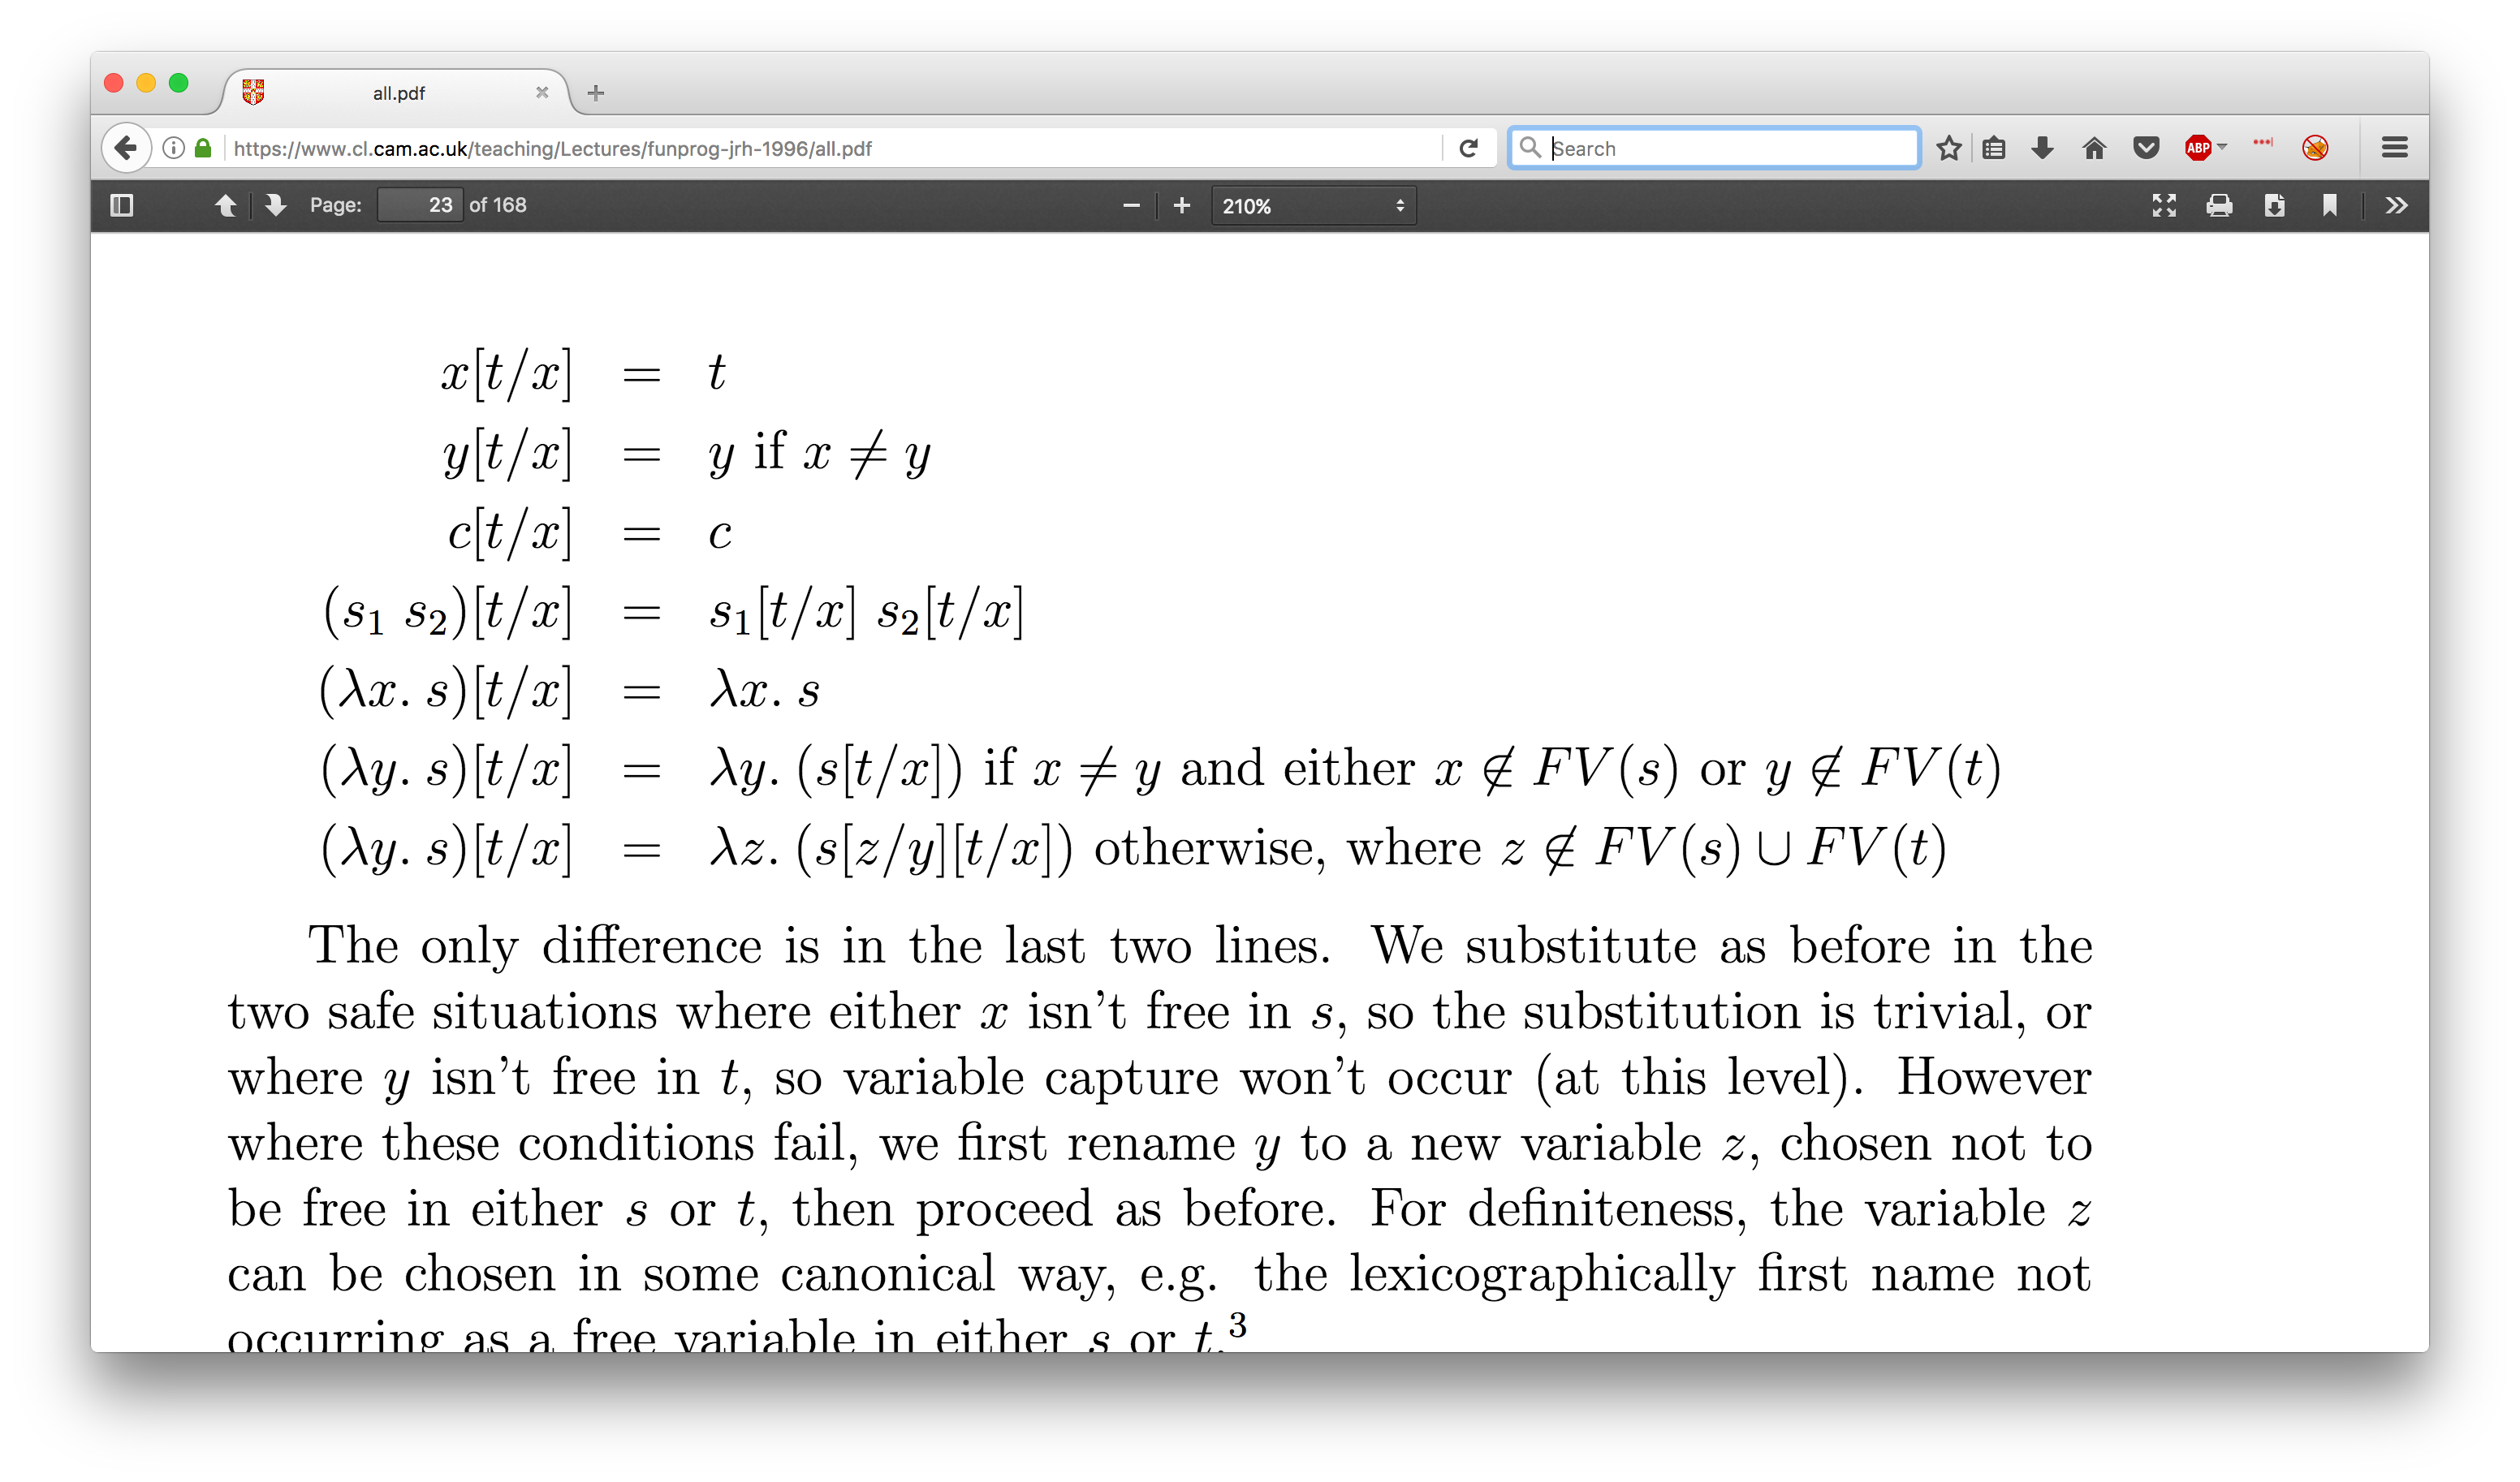
\includegraphics[width=\linewidth]{Images/calculus}
\end{figure}
\end{frame}

\begin{frame}{El cielo de la arquitectura Java}
\huge Pregunta - ¿Como lo alcanzo?
\begin{figure}
	\centering
	
\includegraphics[width=0.6\linewidth]{Images/angel}
\end{figure}
\end{frame}

\begin{frame}{El cielo de la arquitectura Java}
\huge Respuesta - Construyendo una escalera
\begin{figure}
\centering
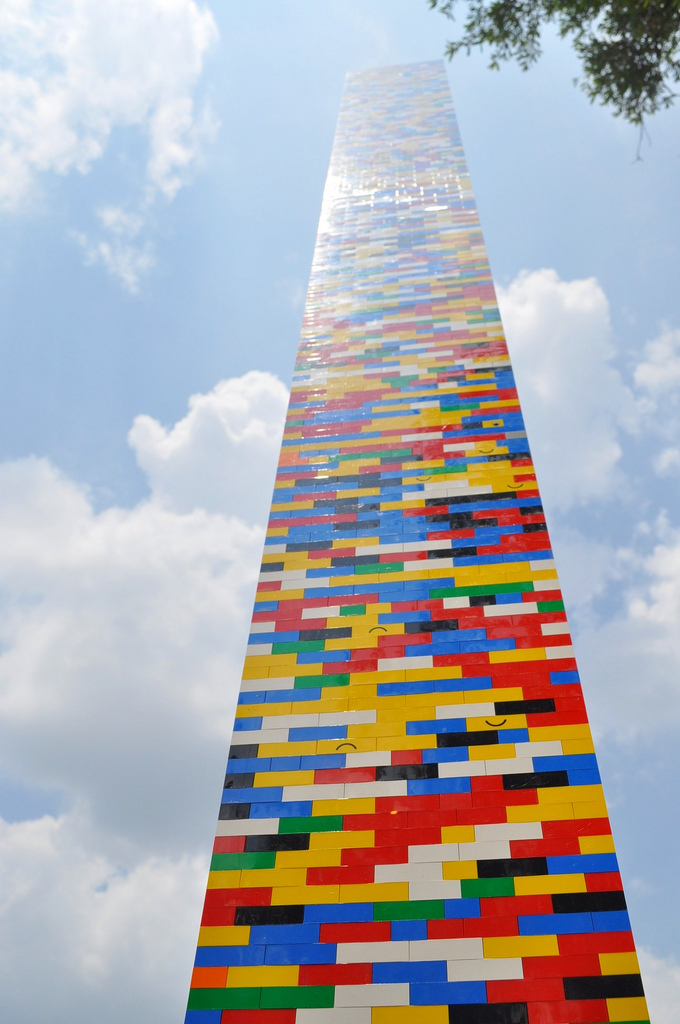
\includegraphics[width=0.6\linewidth]{Images/starwaytoheaven}
\end{figure}
\end{frame}

\begin{frame}{1 - Bloques}
\begin{figure}
\centering
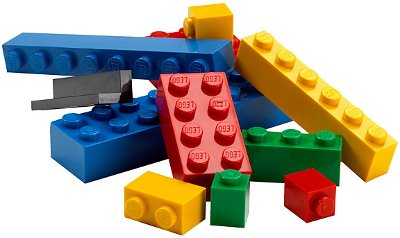
\includegraphics[width=0.9\linewidth]{Images/lego-parts}
\end{figure}
\end{frame}

\begin{frame}{1 - Java 8}
\begin{itemize}
\item Lambda expressions
\item Functional interface
\item High order functions
\item Complements (predicates, method reference)
\end{itemize}
\end{frame}

\begin{frame}{2 - Java Developer Kit Funcional}
\begin{figure}
\centering
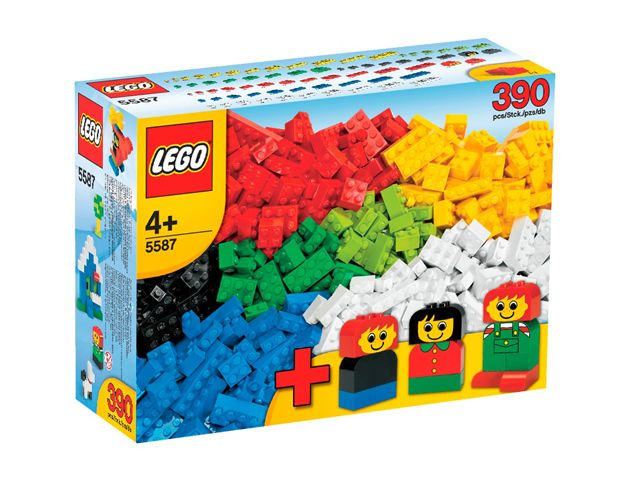
\includegraphics[width=0.9\linewidth]{Images/basic}
\end{figure}
\end{frame}

\begin{frame}{2 - Java Developer Kit Funcional}
\begin{itemize}
\item Funciones predefinidas en Java 8 (java.util.function)
\item Más de 40 interfaces funcionales
\item Streams API
\end{itemize}
\end{frame}


\begin{frame}{3 - Bibliotecas}
\begin{figure}
\centering
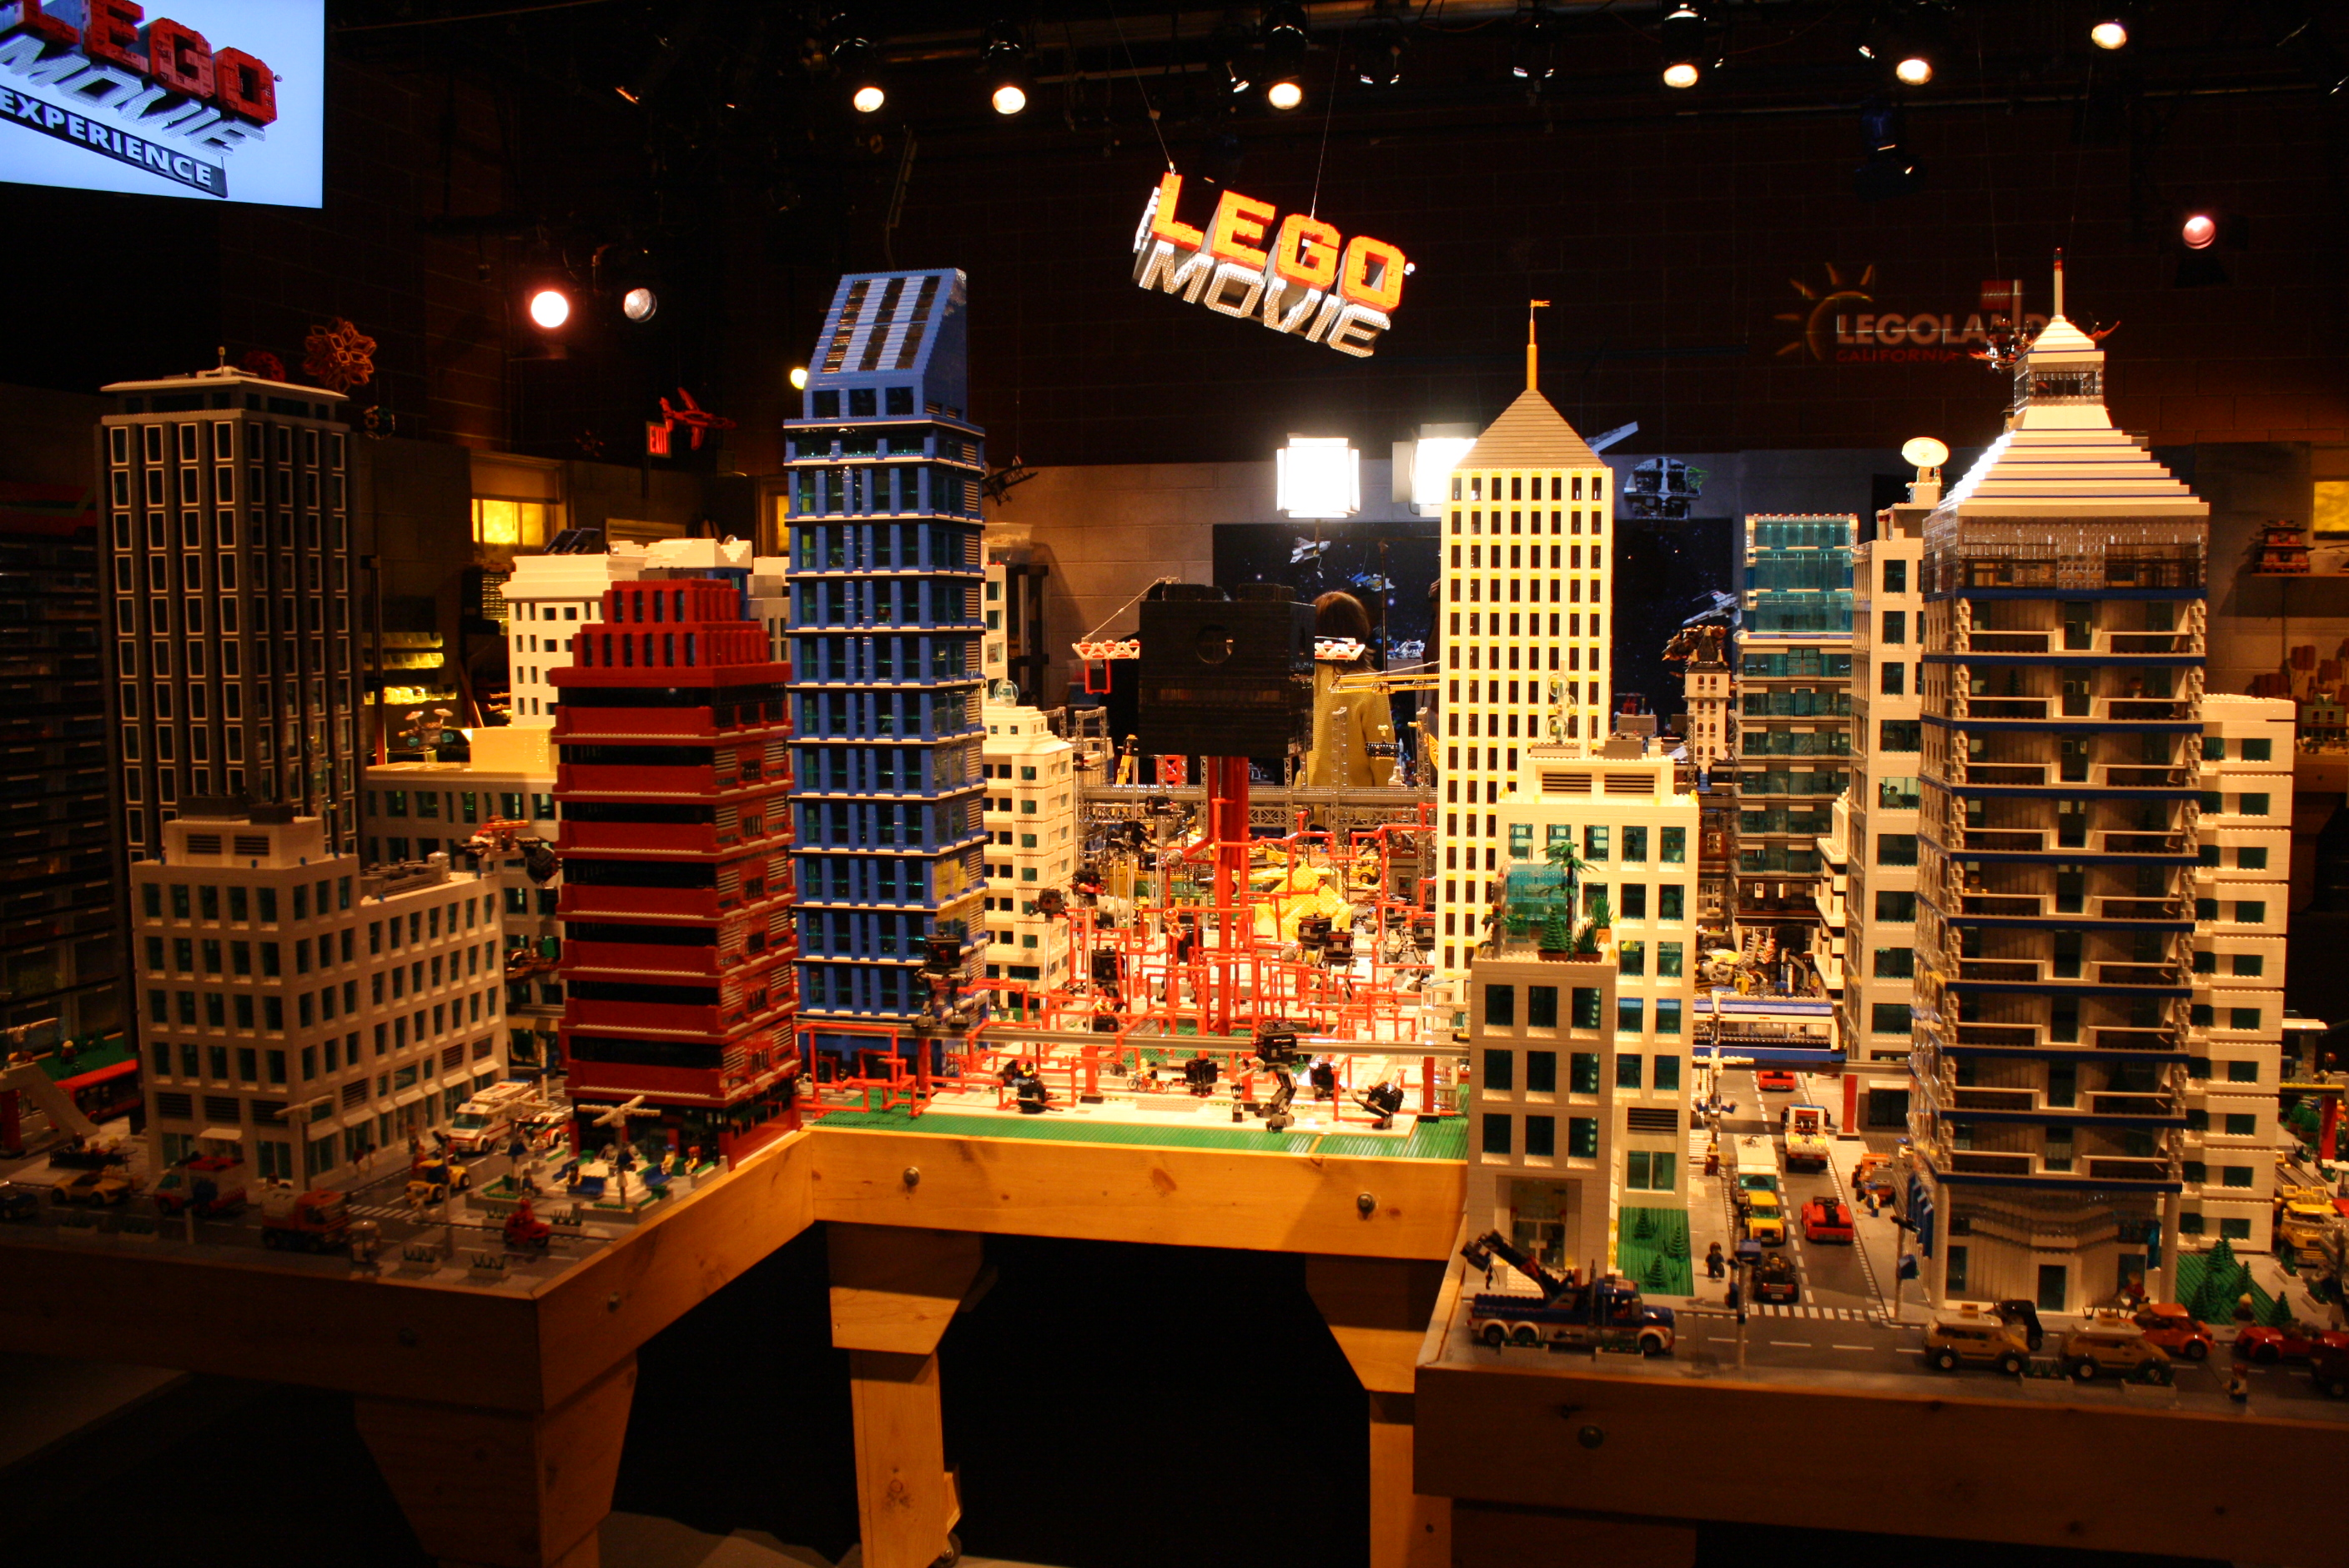
\includegraphics[width=0.9\linewidth]{Images/lego-movie}
\end{figure}
\end{frame}

\begin{frame}{3 - Bibliotecas}
Catedral
\begin{itemize}
\item Java EE (Reactivos)
\item Spring (Reactivos)
\item Lagom (Reactivos)
\end{itemize}

Bazar
\begin{itemize}
\item \textbf{Funcionalidad:} vavr, jOOQ/jOOL, EclipseCollections, FunctionalJava
\item \textbf{Arquitectura:} RxJava, Akka, Vert.x (Interactions - Architecture)
\end{itemize}
\end{frame}

\section{Solución}

\begin{frame}{Solución}
Estado zen del arquitecto de software
\begin{itemize}
	\item \textbf{Productividad} - Java 8
	\item Recurso humano - POO -> Funcional
	\item \textbf{¿Predictibilidad y estabilidad?}
	\item \textbf{¿Escalabilidad?}
	\begin{itemize}
		\item \textbf{App Server} - Vertical y luego horizontal
		\item \textbf{Microservicios} - Horizontal
	\end{itemize}
	\item Costos - Todas las anteriores
\end{itemize}
\end{frame}

\begin{frame}{Solución}
\begin{figure}
	\centering
	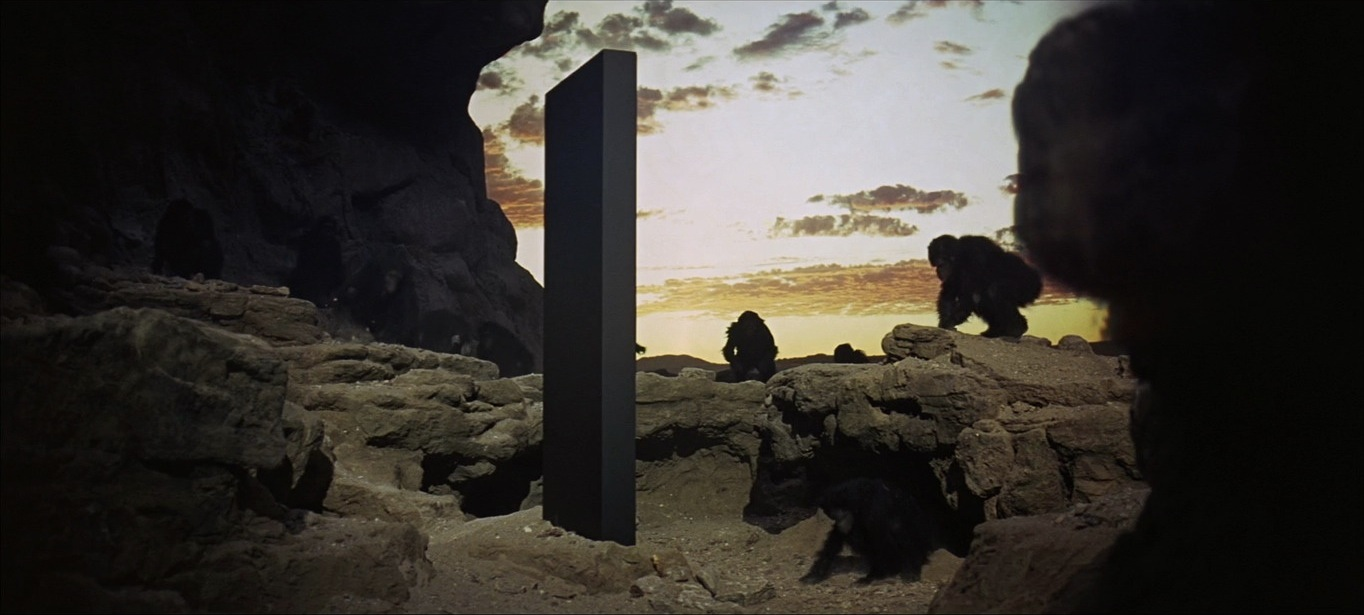
\includegraphics[width=\linewidth]{Images/monolith}
\end{figure}
\end{frame}

\begin{frame}{Monolito}
\begin{figure}
	\centering
	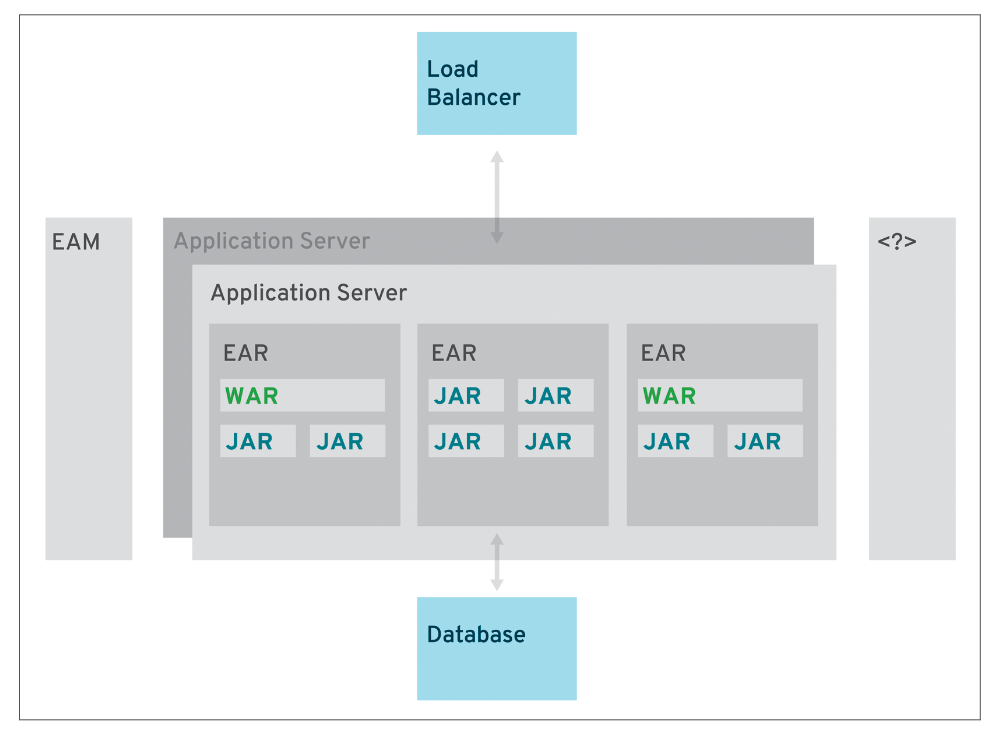
\includegraphics[width=0.7\linewidth]{Images/monolitos}
	\caption{Arquitectura monolitica - Creditos: Markus Eisele}
\end{figure}
\end{frame}

\begin{frame}{ESB}
\begin{figure}
	\centering
	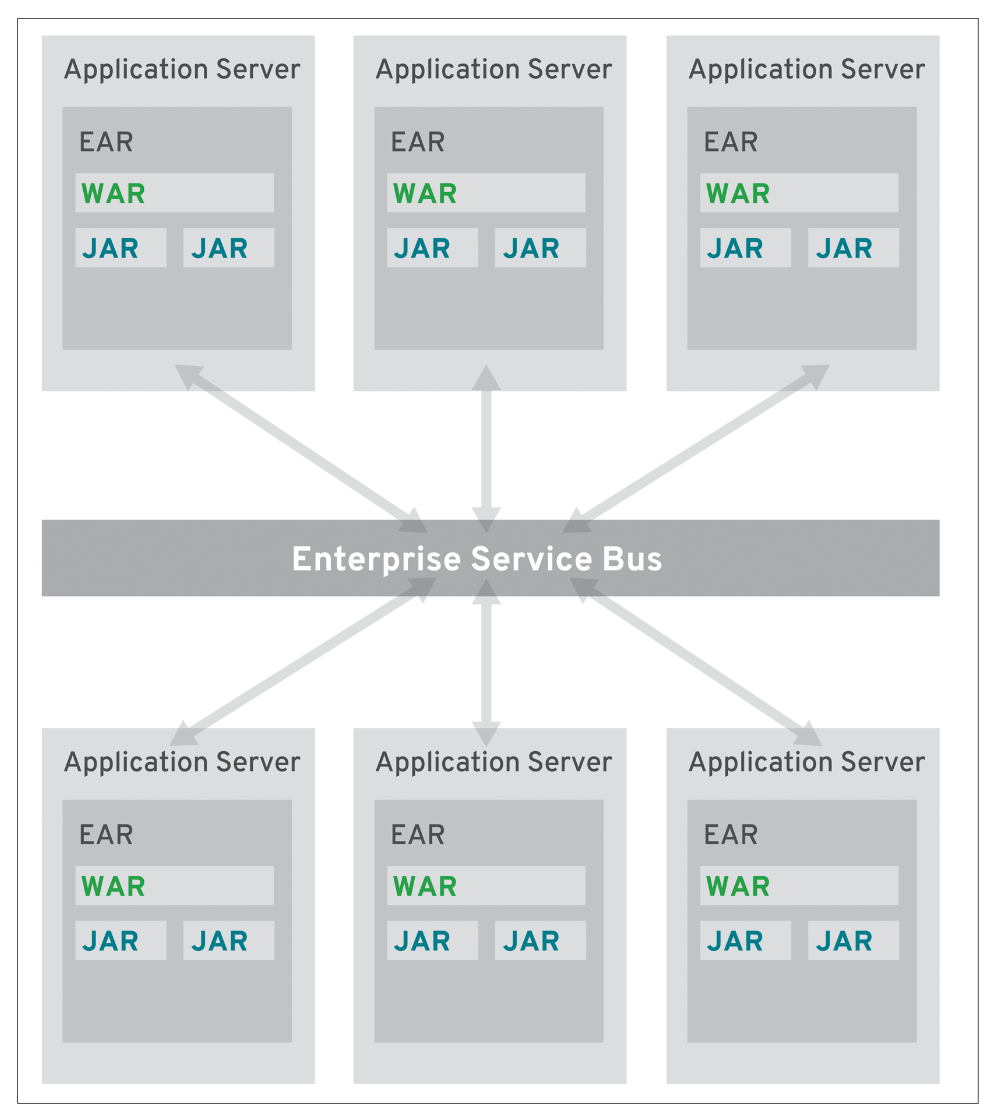
\includegraphics[width=0.5\linewidth]{Images/esb}
	\caption{Arquitectura Esb - Creditos: Markus Eisele}
\end{figure}
\end{frame}

\begin{frame}{Microservicios}
\begin{figure}
	\centering
	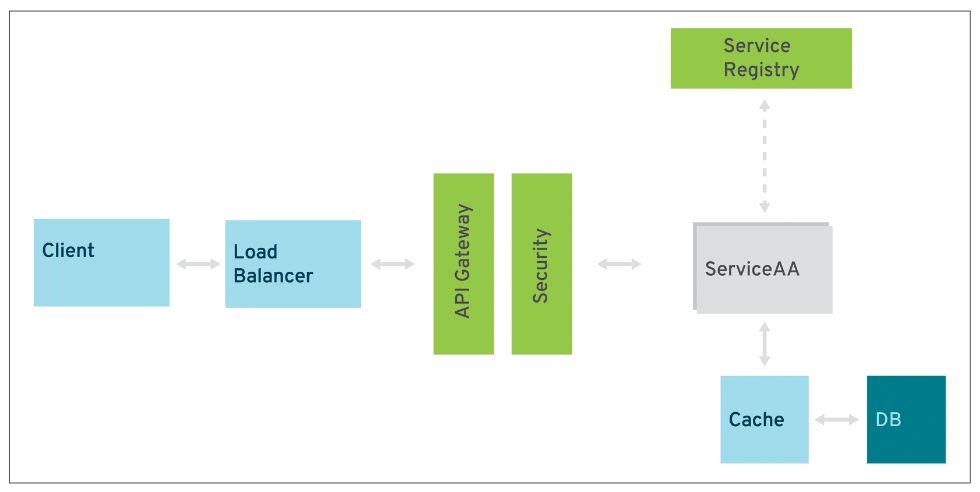
\includegraphics[width=\linewidth]{Images/microservicios}
	\caption{Arquitectura Microservicio - Creditos: Markus Eisele}
\end{figure}
\end{frame}



\begin{frame}{Microservicios}
Ventajas
\begin{itemize}
	\item Bases de código pequeñas
	\item Buenas practicas de programación
	\item Tolerancia a fallas
	\item Escalabilidad
\end{itemize}
Desventajas
\begin{itemize}
	\item Tooling overhead
	\item Debug
	\item Transacciones distribuidas
	\item Latencia
	\item Interdependencia
		\item Falacias de la computación distribuida
\end{itemize}
\end{frame}


\begin{frame}{Microservicios}
Desventaja \\

\huge Hype Driven Development
\end{frame}

\section{Microservicios funcionales con JavaEE}
\begin{frame}{Microservicios - JavaEE}
JavaEE el framework más anti-hype de la tierra\\

\huge J2EE 1.2 (Diciembre 12, 1999)
\end{frame}


\begin{frame}{Microservicios - JavaEE}
Implementación
\begin{itemize}
	\item Refactoring iterativo
	\item Refactoring practico
	\item Nuevos servicios
\end{itemize}
\end{frame}

\begin{frame}{Microservicios - JavaEE}
Implementación
\begin{itemize}
	\item \textbf{Refactoring iterativo}
	\item \textbf{Refactoring practico}
	\item \textbf{Nuevos servicios}
\end{itemize}
\end{frame}

\begin{frame}{Microservicios - JavaEE}
Subset de Api en JavaEE
\begin{itemize}
	\item JAX-RS
	\item JSON-P
	\item CDi, EJB
	\item JCache, JPA
\end{itemize}

Nuevas formas de despliegue
\begin{itemize}
	\item Versiones micro JavaEE (CLI)
	\item Uber-Jar/Fat-Jar/Serverless
\end{itemize}
\end{frame}

\begin{frame}{Microservicios - JavaEE}
Opciones
\begin{itemize}
	\item Wildfly Swarm
	\item KumuluzEE
	\item Dropwizard
	\item WebSphere Liberty
	\item \textbf{Payara Micro}
\end{itemize}

\begin{figure}
	\centering
	
\includegraphics[width=0.5\linewidth]{Images/payaramicro}
\end{figure}
\end{frame}

\begin{frame}{Microservicios - Payara Micro}
\begin{itemize}
	\item Glassfish Embedded (Web Profile)
	\item War en CLI
	\item FatJar en \texttt{main()}
	\item Compatible con Microprofile (JAX-RS, CDI, Config, JSON-P)
	\item JCache y clustering - Hazelcast
\end{itemize}
\end{frame}

\section{Demo}
\begin{frame}{Payara Micro - Demo}
\begin{itemize}
	\item JAX-RS, CDI
	\item DeltaSpike, vavr
	\item JCache
\end{itemize}
\end{frame}

\section{Fin}
\begin{frame}{Gracias}
\begin{itemize}
\item me@vorozco.com
\item http://vorozco.com
\item http://github.com/tuxtor/slides
\end{itemize}
\begin{center}

\includegraphics[width=0.1\linewidth]{Images/cclogo}
\\
This work is licensed under a Creative Commons Attribution-ShareAlike 3.0 Guatemala License.
\end{center}
\end{frame}
\end{document}

